\documentclass[a4paper,12pt]{report}

\usepackage[utf8]{inputenc}
% \usepackage[Vietnamese]{babel}
\usepackage{titling}
%package the indent the first line in latex
\usepackage{indentfirst}
\usepackage{graphicx}
\usepackage{ragged2e}
\usepackage{ragged2e}
\usepackage{afterpage}
\usepackage{amsmath}
\usepackage{subcaption}
\usepackage{float}
\usepackage{alltt}

%adding bibliography
\usepackage[backend=biber]{biblatex}
\addbibresource{/home/pj/MEGA/ComVi/paper_writing/Mendeley/bibitex/library.bib}

\graphicspath{{/home/pj/Documents/proposal/}}
% \graphicspath{{~/coding/python/Music-Sheet-Pitch-Translation/Latex_paper/draft}}

%making the numbering in Roman format 
\renewcommand\thesection{\Roman{section}}
\renewcommand\thesubsection{\roman{subsection}}

\setlength{\droptitle}{-8cm}

\usepackage{tikz}

\pretitle{
    \begin{tikzpicture}[remember picture,overlay]
    \node[anchor=north west,yshift=-1.5pt,xshift=1pt]%
        at (current page.north west)
        {\includegraphics{vgu_logo}};
    \end{tikzpicture}
}
\posttitle{}

\begin{titlepage}
	\title{ MUSIC SHEET UNDERSTANDING AND TONE MODULATION}
	\author{}
\end{titlepage}


\begin{document}

\afterpage{\null\newpage}

\maketitle

\tableofcontents

\clearpage

\section{Research team members}
\begin{itemize}
	\item Team Leader:      \hfill Truong Minh Khoa
	\item Programmer: 		\hfill Dinh Cong Minh
	\item Programmer:		\hfill Nguyen Tho Anh Khoa
	\item Writer/Editor:	\hfill Huynh Minh Triet
\end{itemize}


\section{Disclaimer} 
This report is a product of our team's work, unless otherwise referenced. In
addition, all opinions, results, conclusions, and recommendations are of our own
and may not represent the policies or opinions of the Vietnamese-German
University's Department of Engineering or the University as a whole. 

\clearpage

\section{Abstract}

\section{Introduction}

The topic of recognizing musical sheets, i.e., Optical Music Recognition (OMR),
is not a novel field of research. The term OMR first appeared in a paper written
by MIT scientists in the 60s.  During the last three decades until now, OMR is
an ever increasingly developing field and is capable of solving many problems
that involves with music

More specifically, the current OMR systems of today are capable enough to
recognize a printed musical sheet and digitize it. The resulting output could be
a .midi file, or other types of sound files such as .way, .mp3. The vast
majority of those researches are dedicated for the common user, even for users
who are not educated on musical theory, but there is still a lack of product
that can be used for professional or enthusiast musicians. In reality, a common
problem that is encountered is the modulation of music tones, i.e., up or down
semitone, tone for the whole music sheet. Currently in order to obtain a music
sheet with a few tones higher or lower the musicsian has to manually retype the
entire musical sheet by hand, which is labor intensive.

\subsection{Our solution}
We propose an algorithm that can take in a pdf file or scanned music sheet, then 
translate the written note either by hand or computer drawn into a digital format.
At which stage, the program can play the song or shift the song's tones or semitomes 
according to the musicians' need.

\clearpage

\section{Proposed Method}
The process include first removing the lines on each staff for ease of musical
note dectection.  The second stage is translating the detected note and do note
recognition to translate notes into a digital format. Finnaly the last stage is
where an additional python function will modulate the tones of the song to give
the final output. 


\subsection{Line Removal}
By using the method in \textcite{Gomez2017} the staff's line removal algorithm
will first grayscale the image then invert the color of the image, so that the
lines are now white and the background is black. Finally, using a kernel of the
form: \\
$
\begin{pmatrix}
	0 & 0 & 0\\
	1 & 1 & 1\\
	0 & 0 & 0
\end{pmatrix}
$\\
then run with the dilate() function built-in OpenCV, the horizontal lines will
be expand so that its width is increasingly larger, and any white pixels, i.e.,
notes, that does not belong to the horizontal line, will be flipped to 0 and
becomes the background thus eliminating notes.

result:
\begin{figure}[H]
    \centering
    \begin{subfigure}[t]{0.5\textwidth}
        \centering
        \includegraphics[height=2.0in]{b4_dilate}
        \caption{music sheet before line removal}
    \end{subfigure}%
    ~ 
    \begin{subfigure}[t]{0.5\textwidth}
        \centering
        \includegraphics[height=2.0in]{after_dilate}
        \caption{music sheet after line removal}
    \end{subfigure}
\end{figure}

\clearpage
Finally, flipping the output image will result in a music sheet with lines
removed:
\begin{center}
  \makebox[\textwidth]{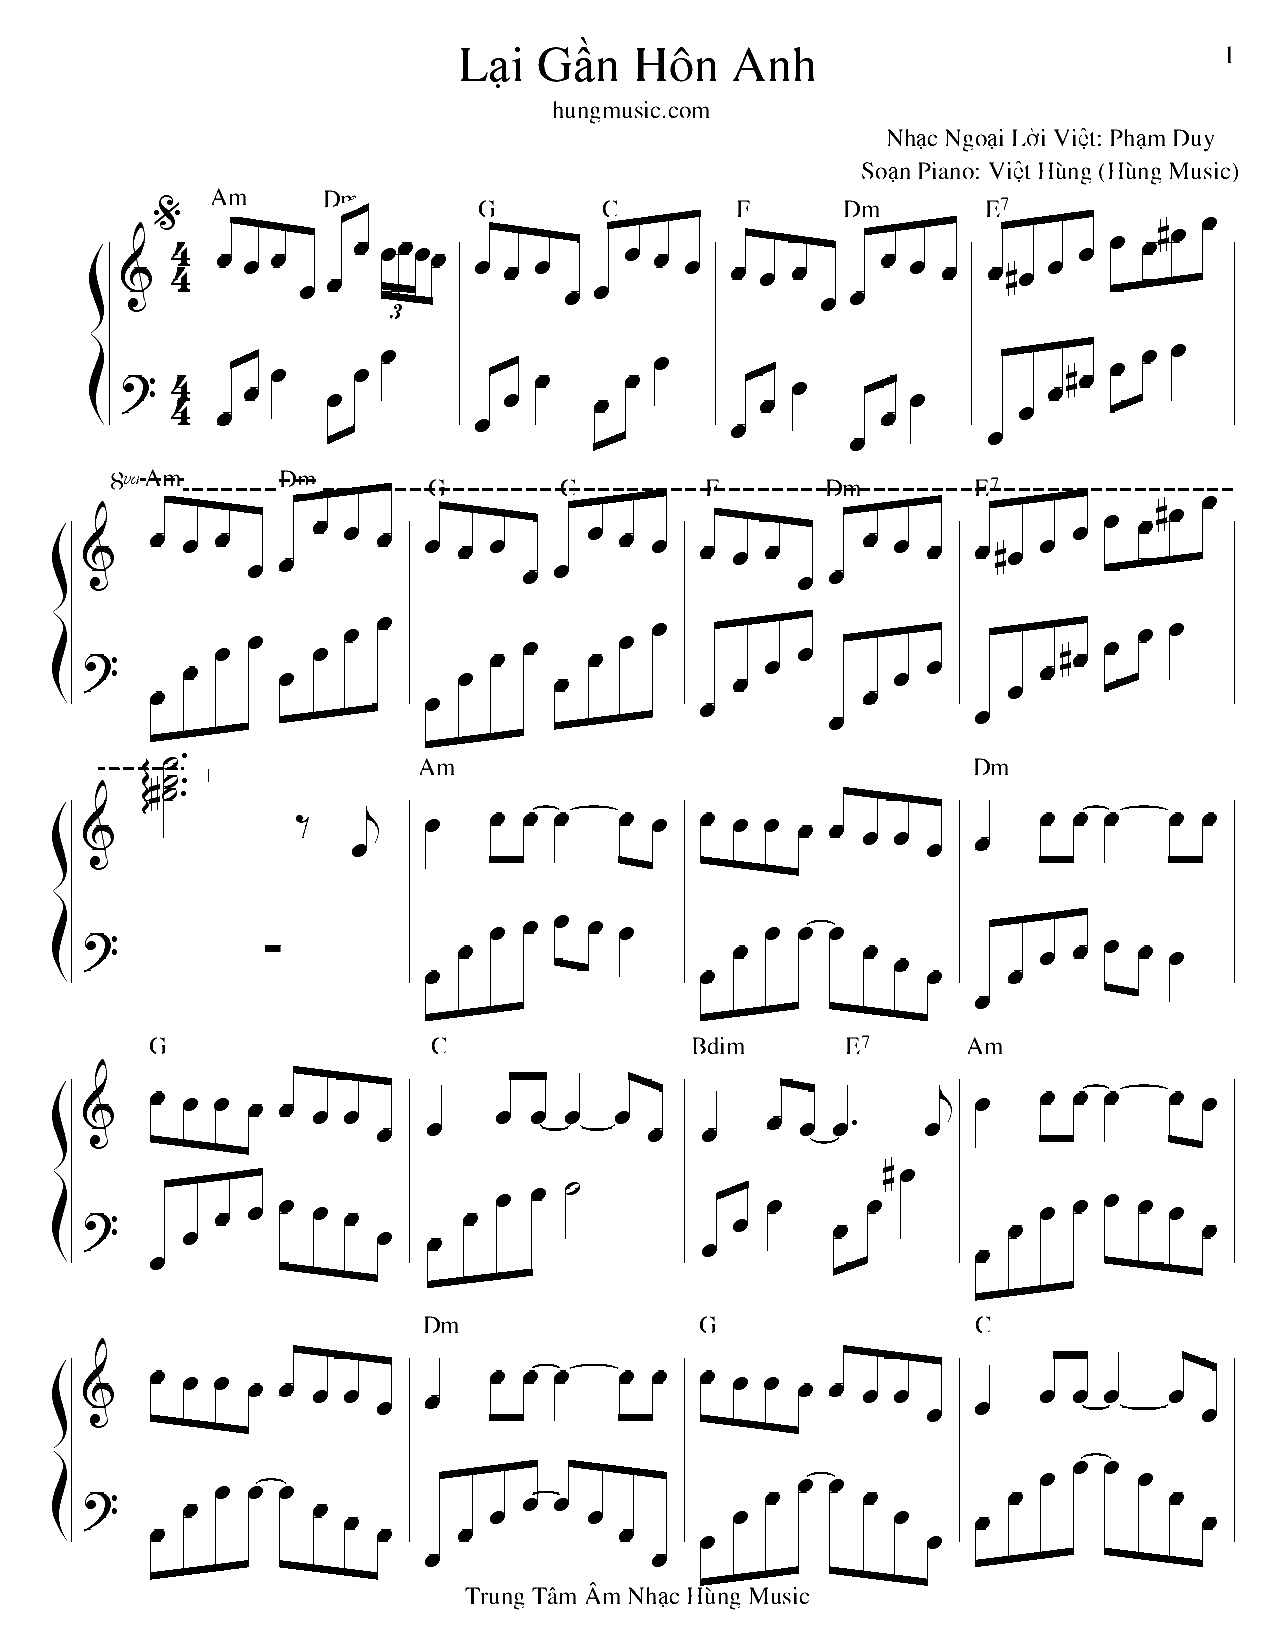
\includegraphics[width=\linewidth]{staffRemoval.jpg}}
\end{center}

\clearpage

\subsection{Note Translation}
In order to translate the note its input as pictorial data to a digitalized form so 
computer can process the music sheet, three steps are required. First by using 
\textcite{Rosebrock} method to eliminate overlaping note positions. Second is to
reorder the notes that are on the same staff lines into a list, for each staff line
there is a corresponding list containing the positions of each note on that staff.
Finally, converting the note positions into musical note notation.

\subsubsection{Eliminating overlaping positions}
By running template matching on the output music sheet that is removed of staff
lines will obtain a list of position of notes on said music sheet. However, 
there is a problem with multiple note positions overlapping each others.\\

Inorder to handle this we use  \textcite{Rosebrock} method call Faster Non
Maxium Supression so that each note will only have one position entry, avoiding
duplication in our list of note positions.\\

\subsubsection{Note reordering}
Next musical notes that belongs to the same staff will begrouped into a same
list.  In order to do this, notes that falls within the range of the first line (the
bottom line) up to the height of half a staff height and and from the last line
(the top line) down to half the height of half a staff height, will be considered
as bellong within the same staff.\\

In musical sheet if two staves are connected with a curly bracket on the left
meaning they must be played simultaneously.

E.g:\\ 
% \includegraphics{two_staff}
\begin{figure}[h]
\makebox[\textwidth]{\includegraphics[width=\linewidth]{two_staff}}
\caption{Two staves that need to be played simultaneously}
\label{fig:two staves}
\end{figure}

In the example above the staff above with the treble clef is called the main
staff and the staff below with the bass clef is called the sub staff. The 
algorithm will now initialize two list MAIN[] and SUB[] to store the two staves
respectively.

\begin{alltt}
    \normalfont
Now the algorithm will move simultaneously through both staff and check the
notes iteratively. For example our first note MAIN[0] and SUB[0], if they are
vertically aligned, meaning that it need to be play simultaneously, the
alogorithm will then move MAIN[0] and SUB[0] to MAIN\_RE\_ORDERED and
SUB\_RE\_ORDERD. By move the algorithm will cut the note position from the
original MAIN list and paste it into the MAIN\_RE\_ORDERED, same goes for
SUB\_RE\_ORDERED.
\end{alltt}

However since some music sheet has minor error in printing resulting in minor
misalignment of the note, meaning they are still supposed to be play
simultaneously but their horizontal (x axis) position are not exactly the
same. The function ReoderedStaffs() has a threshold value of 5, meaning if
the two notes deviate from each other, either to the left or right, less than
5 pixels we will consider that they will be played simultaneously.

If there is a case, where there is only one note on one of the staff, meaning
only one note need to be played at that moment, we will add the tuple (0,0)
into the staff that doesn't have a note as a filler note. In the case that any
staff ran out of note before the other staff, we will continue the moving
process like normal, but will fill in elements (0,0) for the ran out staff.
Doing this assure that the two list MAIN\_RE\_ORDERED and SUB\_RE\_ORDERED will
always have the same number of elements in their list.\\

\noindent This is the result of the first five notes of the two staves in figure number
\ref{fig:two staves}\\

\begin{figure}[H]
\begin{verbatim}
(216, 253), (242, 260), (270, 253), (298, 285), (325, 278)
(216, 412), (271, 368), (298, 381), (0, 0),     (353, 368)
\end{verbatim}
\caption{The fourth position has a (0,0) tuple because there is no corresponding fourth
note on the sub staff}
\end{figure}

\subsubsection{Digitalization of the notes}




\printbibliography

\end{document}
